\documentclass[11pt]{article}

% parameters are fairly self-explanatory here, thankfully
\usepackage[width=7in,height=9.5in,top=0.75in,centering]{geometry}

% for math-ing
\usepackage{amsmath}
\usepackage{amssymb}
\usepackage{comment}

%%%%%% tables %%%%%%%%

\usepackage{array}
\renewcommand{\arraystretch}{1.5}
\setlength{\tabcolsep}{8pt}

%%%%%% plotting %%%%%%

\usepackage[dvipsnames]{xcolor}
\usepackage{tikz}
\usepackage{pgfplots}

\pgfplotsset{every axis/.append style={
                    axis x line=middle,    % put the x axis in the middle
                    axis y line=middle,    % put the y axis in the middle
                    axis line style={<->,color=black}, % arrows on the axis
                    xlabel={$x$},          % default put x on x-axis
                    ylabel={$y$},          % default put y on y-axis
            }}
            
 \pgfplotsset{compat=1.14} % sometimes, everything falls apart without this
 
 %\usepgfplotslibrary{fillbetween} %for shading between curves

%%%%%% commands %%%%%%

% exam heading; course name is first argument, exam information is second argument
\newcommand{\Heading}[2]{
    \fbox{
        {\Large\textbf{#1}}
        }
    \hfill
    \fbox{
        \begin{minipage}{0.2\textwidth}
            \begin{center}
            \textbf{#2}
            \end{center}
        \end{minipage}
    }
    \par\vspace{0.1in}}

% for being lazy while beautifying integrals
\newcommand{\dint}{\displaystyle\int}

% for being lazy while beautifying limits
\newcommand{\dlim}{\displaystyle\lim}

%%%%%% side-by-side minipages %%%%%%
\NewDocumentCommand \mpageT { m m o m m }{%First 2 arguments are width of each minipage. Last 2 are contents of each minipage. Optional is to put something in the middle.
        \IfNoValueTF {#3} {  	
        		\begin{minipage}[t]{#1\textwidth}\vspace{0pt}#4 \end{minipage}\begin{minipage}[t]{#2\textwidth}\vspace{0pt}#5 \end{minipage}
        }
        {
		\begin{minipage}[t]{#1\textwidth}\vspace{0pt}#4 \end{minipage} #3 \begin{minipage}[t]{#2\textwidth}\vspace{0pt}#5 \end{minipage}
        }
}

\usepackage{xparse}
\newcommand{\blue}[1]{{\color{blue}#1}}
\NewDocumentCommand \unlineb { m m g }{% For use in tabular environment
        \IfNoValueTF {#3} {  
            		\underline{ \parbox[c][.25in]{#1in}{\centering \text{\blue{$#2$}}  } } %simulates DJ's \rule[-8pt]{0.75in}{0.4pt}
        }
        {
            		\underline{\parbox[c][#3in][c]{#1in}{\centering \text{\blue{$#2$} } }}
        }
}


%%%%%% stuff %%%%%%

\usepackage{fancyhdr}

%\setcounter{page}{0} % first page is page 0

\parindent0pt % no indent

\fboxsep=0.25cm % little space in fbox border

%%%%%% BEGIN! %%%%%%%

\begin{document}

\pagestyle{fancy}

% record goals here to create sense of transparency

\fancyhead[c]{%
  \ifcase\value{page}
  % empty test for page = 0
  \or {}% 
  \or
  \or {\bf\color{ProcessBlue} F1: Lines \& Slope}% page=1
  \or {\bf\color{ProcessBlue} F2: Exponential and Logarithmic Functions}% page = 2
  \or {\bf\color{RoyalBlue} L2: Evaluating Limits Using Continuity and Forms}% page = 3
  \or {\bf\color{RedOrange} A1: Derivatives and Graphing}% page = 4
  \or {\bf\color{RedOrange} A2: Local and Absolute Extreme Values}% page = 5
  \or {\bf\color{RedOrange} A3: Applied Optimization}% page = 6
  \or {\bf\color{Fuchsia} I2: Properties of Definite Integrals}% page = 7
  % \or {\bf\color{Fuchsia} I3: Antiderivatives and Indefinite Integrals}% page = 8
  % \or {\bf\color{Fuchsia} I4: Compute Definite Integrals}
  \else
  % Empty chead here!
  \fi
}

\thispagestyle{empty} % don't display that this is page 0

\Heading{MATH 1190/1210 Survey of Calculus I}{Final Exam Part 2: Reassement Targets\\Spring 2026}

\vspace{0.1in}

\textbf{Name} \hrulefill \, \begin{minipage}{0.16\textwidth}\begin{center}\textbf{UVA ID\\ (e.g. hdj4nd)} \end{center}\end{minipage}\hrulefill\\

\begin{minipage}{0.2\textwidth}\begin{center}\textbf{Course \&\\ Section Number} \end{center}\end{minipage} \hrulefill\,\,\textbf{Date} \hrulefill  \\

\hrulefill
\paragraph*{Course \& Section Numbers:}

{\small
\begin{center}
\begin{tabular}{| c | c | c | c |}
\hline
\begin{minipage}{0.12\textwidth}\centering
1190-100\\
J. Rolf\\
(2:00 PM)
\end{minipage}
&
\begin{minipage}{0.12\textwidth}\centering
1190-200\\
J. Rolf\\
(3:30 PM)
\end{minipage}
&
\begin{minipage}{0.12\textwidth}\centering
1190-100\\
Michael\\
(11 AM)
\end{minipage}
&
\begin{minipage}{0.12\textwidth}\centering
1210-200\\
Susan\\
(9:30 AM)
\end{minipage}
\\ \hline
\begin{minipage}{0.12\textwidth}\centering
1210-300\\
Susan\\
(2 PM)
\end{minipage}
&
\begin{minipage}{0.12\textwidth}\centering
1210-400\\
Holden\\
(12:30 PM)
\end{minipage}
&
\begin{minipage}{0.12\textwidth}\centering
1210-500\\
Susan\\
(3:30 PM)
\end{minipage}
&
\begin{minipage}{0.12\textwidth}\centering
1210-700\\
Aaratrick\\
(2:00 PM)
\end{minipage}
\\ \hline
\begin{minipage}{0.12\textwidth}\centering
1210-800\\
J. Bowling\\
(3:30 PM)
\end{minipage}
&
\begin{minipage}{0.12\textwidth}\centering
1210-900\\
J. Bowling\\
(5 PM)
\end{minipage}
&
\begin{minipage}{0.12\textwidth}\centering
1210-930\\
Vadim\\
(11 AM)
\end{minipage}
\\
\cline{1-3}
\end{tabular}
\end{center}
}

{%\small

\paragraph*{Instructions:}

\begin{itemize}
    
    \item The regular time allowed for completing this assessment is \fbox{$80$} minutes.
    \item \textbf{This part of the final exam is optional.} It provides one additional opportunity to attempt the following learning targets.
    {\bf\color{ProcessBlue}F1}, {\bf\color{ProcessBlue}F2}, {\bf\color{RoyalBlue}L2}, {\bf\color{RedOrange}A1}, {\bf\color{RedOrange}A2}, {\bf\color{RedOrange}A3}, {\bf\color{Fuchsia}I2}, %{\bf\color{Fuchsia}I3}, {\bf\color{Fuchsia}I4}.
    %\item This assessment is out of 50 points.\\
    \item On each problem, you will receive a score of Exceeds Expectations (5), Proficient (4), Almost (3), Developing (2), Emerging (1), or Not Yet (0). {\bf Please do not interpret your score as a percentage.}
    %\item You will have opportunities to reassess on the targets appearing on this assessment after the next {\bf 2} assessments.\\
    \item You may NOT use calculators, dictionaries, notes, phones, or any other kind of aid.
    \item Please write neatly. What cannot be read, cannot be graded.
    \item Carefully work out each problem and clearly indicate your final answer to every problem.
    \item Throughout, give the most descriptive answer possible. \textbf{For instance, ``DNE" will not be accepted when ``$=\infty$" is applicable.}
    %\item Please provide the most specific answer possible. For instance, if a limit does not exist because it goes to $\infty$ or $-\infty$, then specify this.
    \item Please use the methods discussed up to this point in the course. For example, any work based on l'H\^opital's Rule will not receive credit.
    \item \textbf{All work must be shown unless otherwise specified.} Partial credit will not be given if appropriate work is not shown.
    \item In particular, {\bf any answer appearing with no justification will receive no credit regardless of whether the answer was correct}, unless otherwise specified.
    \item Please first respond to the prompts on which you feel most proficient, then respond to others later.
    \item This booklet is printed double-sided. It contains 12 pages and 7 numbered problems.
    \end{itemize}
    
    }

\vfill


%%%%%%%%%
\newpage

This page is left blank intentionally.\\

Use this page if you need additional space to write your solutions to any problem. \\

If you wish this page graded, you must refer to this page on \textbf{the original page} of the problem. Otherwise, your grader will NOT consider your work on this page.

\newpage%
%%%%%%%%%


\begin{enumerate}

%%%%%%%%%%%%%%%%%%%%%%%%%%%%%%%%%%%%%%%%%%%%%%%%%%%%%
%%%%%%%%%%% BEGIN PROBLEM F1 %%%%%%%%%%%%%%%%%%%%%%%%
%%%%%%%%%%%%%%%%%%%%%%%%%%%%%%%%%%%%%%%%%%%%%%%%%%%%%

\item A demand curve in the stock market describes the relationship between the number of shares $Q$ that investors are willing to purchase and the stock price $P$ (in dollars).\\
\vspace{0.5cm}

\noindent
\begin{minipage}{0.38\textwidth}
\centering
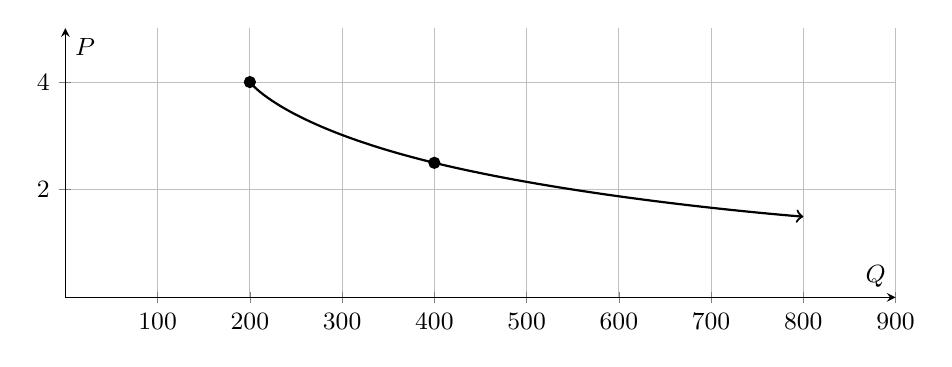
\begin{tikzpicture}
\begin{axis}[
    axis lines=middle,
    xlabel={$Q$},
    ylabel={$P$},
    xmin=0, xmax=900,
    ymin=0, ymax=5,
    grid=both,
    width=\textwidth,
    height=5cm,
    tick label style={font=\small},
    label style={font=\small}
]

\addplot[only marks] coordinates {
    (200,4)
    (400,2.5)
};

% \addplot[thick] coordinates {
%     (200,4)
%     (400,2.5)
%     (800,1.5)
% };
\addplot[thick, smooth, tension=1,->] coordinates {
    (200,4)
    (400,2.5)
    (800,1.5)
};
\end{axis}
\end{tikzpicture}
\end{minipage}
\hfill
\begin{minipage}{0.58\textwidth}
% A portion of the demand curve is given by:
% \[
% (200, 4), \quad (400, 2.5), \quad (800, 1.5)
% \]
\end{minipage}
\text{\small where $Q$ is in number of shares and $P$ is dollars.}

\vspace{0.5em}

A portion of the demand curve for a particular stock is given by the following data points:
\[
(200, 4), \quad (400, 2.5),
\]
% where $Q$ represents the number of shares (in hundreds) and $P$ represents the price per share (in dollars).

\begin{enumerate}
\item[(a)] What is the average rate of change of the stock price as the quantity demanded increases from 200 to 400 shares?
\vspace{2.2cm}


% \item[(b)] Find the equation of the portion of the demand curve for $0 \le Q \le 400$. Express your answer in the form
% \[
% P(Q) = mQ + b.
% \]
% \vspace{2.2cm}

\item[(b)] Write a sentence describing what the slope of the demand curve represents in this stock market context. Be sure to include appropriate units.
\vspace{2.2cm}

\item[(c)] If $\Delta P = -0.5$ dollars as the quantity demanded increases from 400 to 1000 shares. What is the stock price at which investors are willing to purchase 1000 shares?
\end{enumerate}

%%%%%%%%%%%%%%%%%%%%%%%%%%%%%%%%%%%%%%%%%%%%%%%%%%%%%
%%%%%%%%%%% END PROBLEM F1 %%%%%%%%%%%%%%%%%%%%%%%%%%
%%%%%%%%%%%%%%%%%%%%%%%%%%%%%%%%%%%%%%%%%%%%%%%%%%%%%

\newpage

%%%%%%%%%%%%%%%%%%%%%%%%%%%%%%%%%%%%%%%%%%%%%%%%%%%%%
%%%%%%%%%%% BEGIN PROBLEM F2 %%%%%%%%%%%%%%%%%%%%%%%%
%%%%%%%%%%%%%%%%%%%%%%%%%%%%%%%%%%%%%%%%%%%%%%%%%%%%%

\item Respond to the following prompts.

\begin{enumerate}
    \item Evaluate the following expressions. Simplify as much as possible. Your final answer should be a number without any exponential or logarithmic expressions.

    \begin{enumerate}
        \item[(i)] $\dfrac{(-3)^{-62}}{(-3)^{-60}}$

        \vfill

        \item[(ii)] $\log_{2}(\sqrt[3]{2^4})$

        \vfill
    \end{enumerate}

    \item Solve the following equation for $x$. 

    \[\log_{3}(5x - 1)=2\]

    \vfill
\end{enumerate}

%%%%%%%%%%%%%%%%%%%%%%%%%%%%%%%%%%%%%%%%%%%%%%%%%%%%%
%%%%%%%%%%% END PROBLEM F2 %%%%%%%%%%%%%%%%%%%%%%%%%%
%%%%%%%%%%%%%%%%%%%%%%%%%%%%%%%%%%%%%%%%%%%%%%%%%%%%%

\newpage

%%%%%%%%%%%%%%%%%%%%%%%%%%%%%%%%%%%%%%%%%%%%%%%%%%%%%
%%%%%%%%%%% BEGIN PROBLEM L2 %%%%%%%%%%%%%%%%%%%%%%%%
%%%%%%%%%%%%%%%%%%%%%%%%%%%%%%%%%%%%%%%%%%%%%%%%%%%%%

\item Evaluate the following limits using a theorem about continuity or forms.

If you use a theorem about continuity to evaluate a limit, to receive full credit, please provide sufficient explanation for why the theorem can be used. 

If you use a form to evaluate a limit, to receive full credit, please list the form and show all steps. 

There's no need to simplify your final answer.
\vspace{1.5cm}
\begin{enumerate}
    \item $\lim\limits_{x\to\infty}\dfrac{x^3}{e^x + x^3}$ %change to infty/infty,Exponential/polynomial/log?
\hfill Form: \rule[-8pt]{2in}{0.4pt} \quad Limit: \rule[-8pt]{2in}{0.4pt}
    \vfill

    \item $\lim\limits_{x\to 1^+}\dfrac{x}{1-x}$
\hfill Form: \rule[-8pt]{2in}{0.4pt} \quad Limit: \rule[-8pt]{2in}{0.4pt}

    \vfill
\end{enumerate}

%%%%%%%%%%%%%%%%%%%%%%%%%%%%%%%%%%%%%%%%%%%%%%%%%%%%%
%%%%%%%%%%% END PROBLEM L2 %%%%%%%%%%%%%%%%%%%%%%%%%%
%%%%%%%%%%%%%%%%%%%%%%%%%%%%%%%%%%%%%%%%%%%%%%%%%%%%%

\newpage

%%%%%%%%%%%%%%%%%%%%%%%%%%%%%%%%%%%%%%%%%%%%%%%%%%%%%
%%%%%%%%%%% BEGIN PROBLEM A1 %%%%%%%%%%%%%%%%%%%%%%%%
%%%%%%%%%%%%%%%%%%%%%%%%%%%%%%%%%%%%%%%%%%%%%%%%%%%%%
\item 
\begin{enumerate}
\item The graph shown here is the graph of $y=f''$. Write down the $x$-values of all inflection points of $f(x)$ {\em and} explain why these are inflection points.\\
\mpageT{.4}{.6}{
{
\[
\text{Inflection points ($x$-value(s) only): } \unlineb{1.5}{}
\]
}
}{\flushright
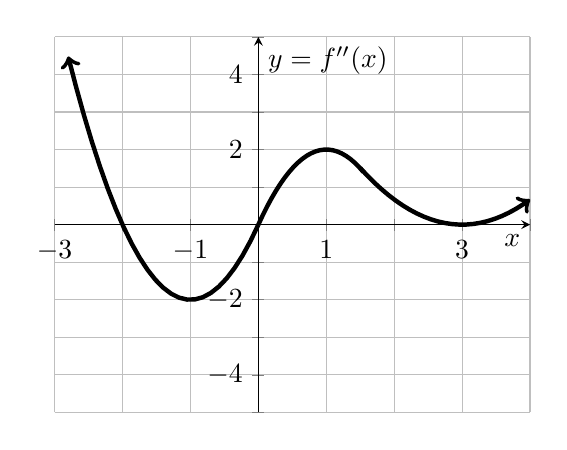
\begin{tikzpicture}
\begin{axis}[
    axis lines=middle,
    xmin=-3, xmax=4,
    ymin=-5, ymax=5,
    ylabel={$y=f^{\prime\prime}(x)$},
    xlabel={$x$},
    xlabel style={anchor=north east},
    grid=both,
    width=3in,
    height=2.5in,
    xtick={-3,-2,-1,1,2,3,4},
    xticklabels={$-3$,,$-1$,$1$,,$3$,},
    ytick={-5,-4,-3,-2,-1,1,2,3,4,5},
    yticklabels={,$-4$,,$-2$,,,$2$,,$4$},
    % legend pos=north west
]
% \addplot[thick, domain=-4:4, samples=200] {(x+2)*x*(x-2)^2/3};
% \addlegendentry{$f''(x)$}
% This is f'(x)
%\addplot[ultra thick, domain=-4:4, samples=200] {(x+2)*x*(x-2)^2/3};
%
% \addplot[domain=-1:3, ultra thick, red] {-(x-2)^2};
          \addplot[domain=1.5:4, ultra thick,->] {.67*(x-3)^2};
          \addplot[domain=0:1.55, ultra thick] {-2*(x-1)^2+2};
          \addplot[domain=-2.8:0, ultra thick,<-] {2*(x+1)^2-2};
%\node at (rel axis cs:0.9,0.15) {$f''(x)$};
\end{axis}
\end{tikzpicture}
}
%\begin{tikzpicture}
%\begin{axis}[
%    axis lines=middle,
%    xmin=-3, xmax=3,
%    ymin=-5, ymax=5,
%    ylabel={$y=f^{\prime\prime}(x)$},
%    grid=both,
%    width=3in,
%    height=2.5in,
%    xtick={-3,-2,-1,1,2,3},
%    xticklabels={$-3$,,$-1$,$1$,,$3$},
%    ytick={-5,-4,-3,-2,-1,1,2,3,4,5},
%    yticklabels={,$-4$,,$-2$,,,$2$,,$4$},
%    % legend pos=north west
%]
%% \addplot[thick, domain=-4:4, samples=200] {(x+2)*x*(x-2)^2/3};
%% \addlegendentry{$f''(x)$}
%% This is f'(x)
%\addplot[ultra thick, domain=-4:4, samples=200] {(x+2)*x*(x-2)^2/3};
%%\node at (rel axis cs:0.9,0.15) {$f''(x)$};
%\end{axis}
%\end{tikzpicture}
%}
\vfill

\mpageT{.6}{.4}{
\item  Continue to assume that the graph shown above is the graph of $y=f''$. Write down the intervals where $f(x)$ is concave down  {\em and} explain why $f(x)$ is concave down on those intervals.
{$\text{Intervals: } \unlineb{1.5}{} $}
}{
\flushright
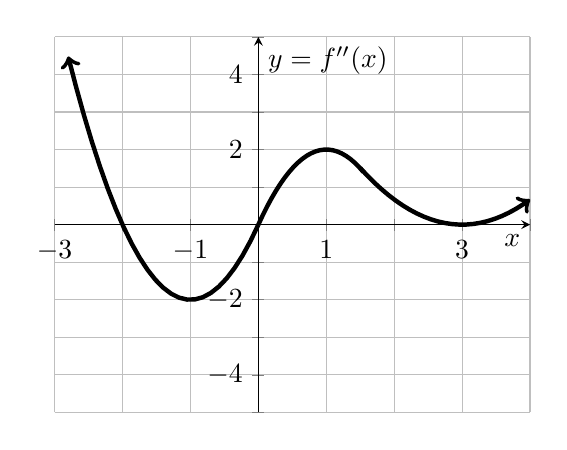
\begin{tikzpicture}
\begin{axis}[
    axis lines=middle,
    xmin=-3, xmax=4,
    ymin=-5, ymax=5,
    ylabel={$y=f^{\prime\prime}(x)$},
    xlabel={$x$},
    xlabel style={anchor=north east},
    grid=both,
    width=3in,
    height=2.5in,
    xtick={-3,-2,-1,1,2,3,4},
    xticklabels={$-3$,,$-1$,$1$,,$3$,},
    ytick={-5,-4,-3,-2,-1,1,2,3,4,5},
    yticklabels={,$-4$,,$-2$,,,$2$,,$4$},
    % legend pos=north west
]
% \addplot[thick, domain=-4:4, samples=200] {(x+2)*x*(x-2)^2/3};
% \addlegendentry{$f''(x)$}
% This is f'(x)
%\addplot[ultra thick, domain=-4:4, samples=200] {(x+2)*x*(x-2)^2/3};
%
% \addplot[domain=-1:3, ultra thick, red] {-(x-2)^2};
          \addplot[domain=1.5:4, ultra thick,->] {.67*(x-3)^2};
          \addplot[domain=0:1.55, ultra thick] {-2*(x-1)^2+2};
          \addplot[domain=-2.8:0, ultra thick,<-] {2*(x+1)^2-2};
%\node at (rel axis cs:0.9,0.15) {$f''(x)$};
\end{axis}
\end{tikzpicture}
}
\vfill

%\begin{flushleft}
%\begin{tikzpicture}
%\begin{axis}[
%    axis lines=middle,
%    xmin=-4, xmax=4,
%    ymin=-6, ymax=6,
%    grid=both,
%    width=3.5in,
%    height=2.5in,
%    xtick={-3,-2,-1,0,1,2,3},
%    ytick={-5,-3,-1,1,3,5},
%    % legend pos=north west
%]
%
%% \addplot[thick, domain=-4:4, samples=200] {(x+2)*x*(x-2)^2/3};
%% \addlegendentry{$f''(x)$}
%% This is f'(x)
%\addplot[thick, domain=-4:4, samples=200] {(x+2)*x*(x-2)^2/3};
%\node at (rel axis cs:0.9,0.15) {$f'(x)$};
%
%\end{axis}
%\end{tikzpicture}
%\end{flushleft}
\vfill 
\mpageT{.6}{.4}{
\item The graph now depicts $f'$.  Write down the interval(s) where $f(x)$ is decreasing {\em and} explain why $f(x)$ is decreasing on those interval(s).\\
{$\text{Intervals: } \unlineb{1.5}{} $}
}{
\flushright
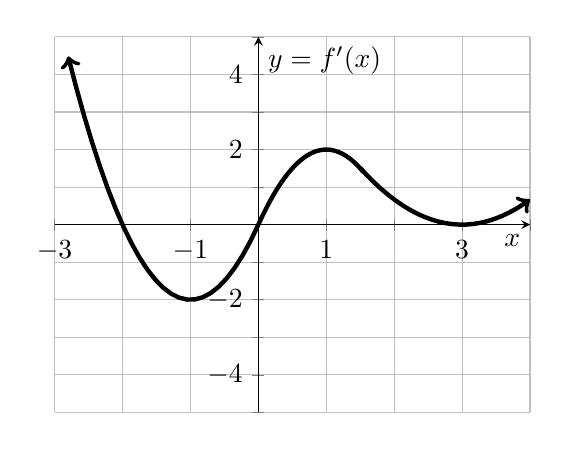
\begin{tikzpicture}
\begin{axis}[
    axis lines=middle,
    xmin=-3, xmax=4,
    ymin=-5, ymax=5,
    ylabel={$y=f^{\prime}(x)$},
    xlabel={$x$},
    xlabel style={anchor=north east},
    grid=both,
    width=3in,
    height=2.5in,
    xtick={-3,-2,-1,1,2,3,4},
    xticklabels={$-3$,,$-1$,$1$,,$3$,},
    ytick={-5,-4,-3,-2,-1,1,2,3,4,5},
    yticklabels={,$-4$,,$-2$,,,$2$,,$4$},
    % legend pos=north west
]
% \addplot[thick, domain=-4:4, samples=200] {(x+2)*x*(x-2)^2/3};
% \addlegendentry{$f''(x)$}
% This is f'(x)
%\addplot[ultra thick, domain=-4:4, samples=200] {(x+2)*x*(x-2)^2/3};
%
% \addplot[domain=-1:3, ultra thick, red] {-(x-2)^2};
          \addplot[domain=1.5:4, ultra thick,->] {.67*(x-3)^2};
          \addplot[domain=0:1.55, ultra thick] {-2*(x-1)^2+2};
          \addplot[domain=-2.8:0, ultra thick,<-] {2*(x+1)^2-2};
%\node at (rel axis cs:0.9,0.15) {$f''(x)$};
\end{axis}
\end{tikzpicture}
}



\vfill
\vfill

\end{enumerate}

%%%%%%%%%%%%%%%%%%%%%%%%%%%%%%%%%%%%%%%%%%%%%%%%%%%%%
%%%%%%%%%%% END PROBLEM A1 %%%%%%%%%%%%%%%%%%%%%%%%%%
%%%%%%%%%%%%%%%%%%%%%%%%%%%%%%%%%%%%%%%%%%%%%%%%%%%%%

\newpage

%%%%%%%%%%%%%%%%%%%%%%%%%%%%%%%%%%%%%%%%%%%%%%%%%%%%%
%%%%%%%%%%% BEGIN PROBLEM A2 %%%%%%%%%%%%%%%%%%%%%%%%
%%%%%%%%%%%%%%%%%%%%%%%%%%%%%%%%%%%%%%%%%%%%%%%%%%%%%

\item Consider the following function $f(x)$.% and its derivative.

\[f(x)=x^{4}-8x^{2}\]%x^3-3x^2+1\]%-(x-1)^4(15x^2+18x+7)\]

%\[f'(x)=10(1-x)^3(3x+1)^2\]

You are required to use methods we've learned in our course, such as the first derivative test, the second derivative test, the closed interval method, or the first derivative test for absolute extrema, to solve this problem. In addition, you need to make sure the method you use is suitable for the question.

\begin{enumerate}
    \item Find all critical numbers of $f(x)$.

    \vfill

    %\item For each critical number found in part (a), classify it as a local minimum, a local maximum, or neither. Fully justify your work.

    %\vfill

    \item Find the $x$-values of all absolute extrema of $f(x)$ on the interval $[-2, 8]$.


    \vfill
\end{enumerate}

%%%%%%%%%%%%%%%%%%%%%%%%%%%%%%%%%%%%%%%%%%%%%%%%%%%%%
%%%%%%%%%%% END PROBLEM A2 %%%%%%%%%%%%%%%%%%%%%%%%%%
%%%%%%%%%%%%%%%%%%%%%%%%%%%%%%%%%%%%%%%%%%%%%%%%%%%%%

\newpage

%%%%%%%%%%%%%%%%%%%%%%%%%%%%%%%%%%%%%%%%%%%%%%%%%%%%%
%%%%%%%%%%% BEGIN PROBLEM A3 %%%%%%%%%%%%%%%%%%%%%%%%
%%%%%%%%%%%%%%%%%%%%%%%%%%%%%%%%%%%%%%%%%%%%%%%%%%%%%

\item A company must produce a sturdy rectangular container with a square base, square top and a volume of $8$ cubic feet. Let $x$ represent the side length of the square base (in feet) and let $h$ represent the height of the box (in feet). Find the dimensions of the box that will minimize the total surface area.\\
\mpageT{.6}{.4}{
To receive full credit, make sure to fully justify why the dimensions you've found maximizes the area. 
%
You are required to use a method we've learned in our course, such as the first derivative test, the second derivative test, the close interval method, or the first derivative test for absolute extrema, as a part of your justification. In addition, you need to make sure the method you use is suitable for the question.
}{
\centering
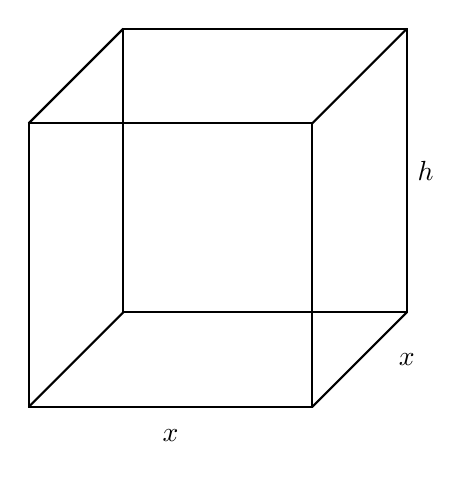
\begin{tikzpicture}[scale=1.2]
% Define coordinates
\coordinate (A) at (0,0);
\coordinate (B) at (3,0);
\coordinate (C) at (3,3);
\coordinate (D) at (0,3);
%
\coordinate (E) at (1,1);
\coordinate (F) at (4,1);
\coordinate (G) at (4,4);
\coordinate (H) at (1,4);
% Draw bottom square
\draw[thick] (A) -- (B) -- (C) -- (D) -- cycle;
% Draw top square
\draw[thick] (E) -- (F) -- (G) -- (H) -- cycle;
% Connect edges
\draw[thick] (A) -- (E);
\draw[thick] (B) -- (F);
\draw[thick] (C) -- (G);
\draw[thick] (D) -- (H);
% Labels
\node at (1.5,-0.3) {$x$};
\node at (4,0.5) {$x$};
\node at (4.2,2.5) {$h$};
\end{tikzpicture}
}
\vspace{0.5cm}



% \begin{enumerate}
%     \item Write an expression for the volume constraint relating $x$ and $h$.

%     \vfill

%     \item Write a function $C(x)$ that represents the total cost of producing the box.

%     \vfill
%     \item Write the domain of this function.
%     \vfill

%     \item Find the value of $x$ that minimizes the cost.

%     \vfill

%     \item Find the corresponding height $h$.

%     \vfill
% \end{enumerate}
%%%%%%%%%%%%%%%%%%%%%%%%%%%%%%%%%%%%%%%%%%%%%%%%%%%%%
%%%%%%%%%%% END PROBLEM A3 %%%%%%%%%%%%%%%%%%%%%%%%%%
%%%%%%%%%%%%%%%%%%%%%%%%%%%%%%%%%%%%%%%%%%%%%%%%%%%%%

\newpage

%%%%%%%%%%%%%%%%%%%%%%%%%%%%%%%%%%%%%%%%%%%%%%%%%%%%%
%%%%%%%%%%% BEGIN PROBLEM I2 %%%%%%%%%%%%%%%%%%%%%%%%
%%%%%%%%%%%%%%%%%%%%%%%%%%%%%%%%%%%%%%%%%%%%%%%%%%%%%

\item The graph of $h(x)$ is given below.

\begin{center}
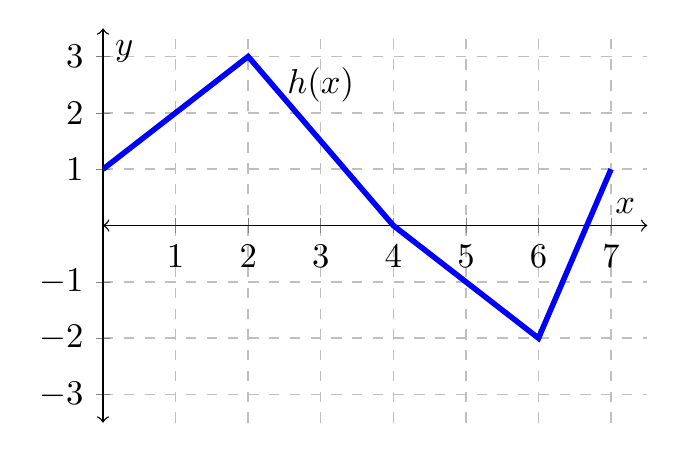
\begin{tikzpicture}[scale=1.25]
\begin{axis}[
    xlabel={$x$},
    xtick={0,1,2,3,4,5,6,7},
    ytick={-3,-2,-1,0,1,2,3},
    xmin=0, xmax=7.5,
    ymin=-3.5, ymax=3.5,
    grid=both, grid style=dashed,
    height=2.2in, width=2.8in
]

% Piecewise linear graph
\draw[ultra thick, blue]
(0,1) -- (2,3) -- (4,0) -- (6,-2) -- (7,1);

\node at (3,2.5) {$h(x)$};

\end{axis}
\end{tikzpicture}
\end{center}

In addition, a function $k(x)$ satisfies:

\[
\int_6^4 k(x)\,dx = -6
\]

\[
\int_2^4 k(x)\,dx = 4
\]

Find the values of the following integrals.

\begin{enumerate}

\item $\displaystyle\int_2^6 h(x)\,dx$

\vfill

\item $\displaystyle\int_2^6 \big(20h(x) - k(x)\big)\,dx$

\vfill

% \item $\displaystyle\int_0^6 \big(2h(x) - k(x)\big)\,dx$

% \vfill

\end{enumerate}
%%%%%%%%%%%%%%%%%%%%%%%%%%%%%%%%%%%%%%%%%%%%%%%%%%%%%
%%%%%%%%%%% END PROBLEM I2 %%%%%%%%%%%%%%%%%%%%%%%%%%
%%%%%%%%%%%%%%%%%%%%%%%%%%%%%%%%%%%%%%%%%%%%%%%%%%%%%

\newpage
\begin{comment}
%%%%%%%%%%%%%%%%%%%%%%%%%%%%%%%%%%%%%%%%%%%%%%%%%%%%%
%%%%%%%%%%% BEGIN PROBLEM I3 %%%%%%%%%%%%%%%%%%%%%%%%
%%%%%%%%%%%%%%%%%%%%%%%%%%%%%%%%%%%%%%%%%%%%%%%%%%%%%

\item Assume $x>0$. Write down the indefinite integrals of the following expressions. 

Although no work is required, you are encouraged to include any work that shows your thought process. 

%constant, power, exponential, log, +C, algebraic manipulation

\begin{center}
        \begin{tabular}{l c r l c r}
            %
            $\displaystyle\int x^{19}\,dx$ & $=$ & \rule[-8pt]{1.5in}{0.4pt} &
            %
            $\displaystyle\int \dfrac{1}{x^3} \,dx$ & $=$ & \rule[-8pt]{1.5in}{0.4pt}\\[1in]
            %%%%%
            $\displaystyle\int \dfrac{5}{x}-5\,dx$ & $=$ & \rule[-8pt]{1.5in}{0.4pt}&
            %
            $\displaystyle\int 7^x\,dx$ & $=$ & \rule[-8pt]{1.5in}{0.4pt}\\[1in]
            %%%%%
            $\displaystyle\int 2e^x+\sqrt[4]{x} \,dx$ & $=$ & \rule[-8pt]{1.5in}{0.4pt} & 
            %
            $\displaystyle\int \dfrac{1}{\sqrt{x^3}} \,dx$ & $=$ & \rule[-8pt]{1.5in}{0.4pt}\\[0.3in]
            %%%%%
        \end{tabular}
\end{center}

%%%%%%%%%%%%%%%%%%%%%%%%%%%%%%%%%%%%%%%%%%%%%%%%%%%%%
%%%%%%%%%%% END PROBLEM I3 %%%%%%%%%%%%%%%%%%%%%%%%%%
%%%%%%%%%%%%%%%%%%%%%%%%%%%%%%%%%%%%%%%%%%%%%%%%%%%%%

\newpage

%%%%%%%%%%%%%%%%%%%%%%%%%%%%%%%%%%%%%%%%%%%%%%%%%%%%%
%%%%%%%%%%% BEGIN PROBLEM I4 %%%%%%%%%%%%%%%%%%%%%%%%
%%%%%%%%%%%%%%%%%%%%%%%%%%%%%%%%%%%%%%%%%%%%%%%%%%%%%

\item For each of the following definite integrals, determine whether the Fundamental Theorem of Calculus (FTC) can be applied to evaluate. 

If so, evaluate the integral using the FTC. There's no need to simplify your final answer.

If not, clearly indicate that and explain why.

\begin{enumerate}
    \item $\displaystyle\int_{-1}^{3}6x^2+\sqrt{x}-1\, dx$

    \vfill

    \item $\displaystyle\int_{1}^3\dfrac{1}{x}-e^x+4\, dx$

    \vfill
\end{enumerate}

%%%%%%%%%%%%%%%%%%%%%%%%%%%%%%%%%%%%%%%%%%%%%%%%%%%%%
%%%%%%%%%%% END PROBLEM I4 %%%%%%%%%%%%%%%%%%%%%%%%%%
%%%%%%%%%%%%%%%%%%%%%%%%%%%%%%%%%%%%%%%%%%%%%%%%%%%%%
\end{comment}
\newpage

\begin{center}
{\bf DO NOT REMOVE THIS SHEET FROM YOUR EXAM PACKET}
\end{center}

\begin{center}
    \begin{tabular}{ r | c | l }
    {\bf Description} & {\bf Formula} & {\bf Variables}\\
    \hline
    area of a square & $A=s^2$ & $s=$ side length\\
    \hline
    area of a rectangle & $A=lw$ & $l=$ length, $w=$ width\\
    \hline
    area of a triangle & $A=\frac12bh$ & $b=$ base, $h=$ height\\
    \hline
    area of a circle & $A=\pi r^2$ & $r=$ radius\\
    \hline
    volume of a rectangular box & $V=lwh$ & $l=$ length, $w=$ width, $h=$ height\\
    \hline
    %volume of a circular cylinder & $V=\pi r^2 h$ & $r=$ radius, $h=$ height\\
    %\hline
    %volume of a sphere & $V=\frac43\pi r^3$ & $r=$ radius\\
    %\hline
    revenue & $R(x) = p\cdot x = p\cdot Q$ & $p=$ unit price, $x=Q=$ quantity sold\\
    \hline
    profit & $P(x) = R(x) - C(x)$ & $R(x)=$ revenue, $C(x)=$ cost\\
    \hline
    average cost & $\overline C(x) = \frac{C(x)}{x}$ & $C(x)=$ cost\\
    \end{tabular}
\end{center}

\begin{center}
{\bf DO NOT REMOVE THIS SHEET FROM YOUR EXAM PACKET}
\end{center}

\newpage

This page is left blank intentionally.\\

Use this page if you need additional space to write your solutions to any problem. \\

If you wish this page graded, you must refer to this page on \textbf{the original page} of the problem. Otherwise, your grader will NOT consider your work on this page.

\newpage

This page is left blank intentionally.\\

Use this page if you need additional space to write your solutions to any problem. \\

If you wish this page graded, you must refer to this page on \textbf{the original page} of the problem. Otherwise, your grader will NOT consider your work on this page.

\end{enumerate}

\end{document}